\documentclass[10pt,a4paper]{article}
\usepackage[utf8]{inputenc}
\usepackage[english,russian]{babel}
\usepackage[OT1]{fontenc}
\usepackage{amsmath}
\usepackage{amsfonts}
\usepackage{amssymb}
\usepackage{graphicx}
\usepackage{float}
\usepackage{wrapfig}
\usepackage{caption}
\DeclareCaptionLabelSeparator{dot}{. }
\captionsetup{justification=centering,labelsep=dot}
\graphicspath{{pictures/}}
\DeclareGraphicsExtensions{.pdf,.png,.jpg,.eps}
\begin{document}

\part{Основы}

\textbf{\Large1 Введение}\\

\textbf{1.1 Значение неопределённости в робототехнике}\\

Робототехника – это область знаний, изучающая   манипулирование предметами физического мира и его восприятие с помощью устройств, управляемых компьютером. Примеры успешного применения робототехнических систем включают автономные платформы для исследований других планет, промышленные манипуляторы на производственных линиях, автомашины, которые могут двигаться без участия водителя и медицинские роботы для помощи хирургам при выполнении операций. Робототехнические системы действуют в физическом мире, воспринимают информацию об окружающем с помощью датчиков и воздействуют на предметы с помощью физических сил.

Хотя робототехника, в большей степени, все ещё проходит период становления, идея манипулирования объектами, используя «умные» устройства, имеет невероятный потенциал, способный изменить жизнь всего человечества. Разве не станет лучше, если все наши автомобили приобретут возможность безопасно передвигаться самостоятельно, сделав дорожно-транспортные происшествия лишь достоянием истории? И если роботы, вместо людей, будут очищать зоны радиоактивных катастроф, таких, как Чернобыль?
И только представьте, что будет, если наши жилища будут населены умными помощниками, которые позаботятся обо всем, что связано с обслуживанием и ремонтом дома? 

Чтобы выполнять такие задачи, роботам необходимо суметь приспособиться к невероятно высокой степени неопределённости, которая существует в физическом мире. C точки зрения робота, имеется целый ряд факторов, вносящих вклад в увеличение неопределённости.

Во-первых, и прежде всего, по определению непредсказуема \textit{окружающая среда}, в которой действует робот. Хотя степень неопределённости в хорошо организованных средах, таких, как сборочные конвейеры, достаточно мала, условия на шоссе и в частных домах очень динамично, и, во многом, непредсказуемым образом изменяются. Степень неопределённости особенно высока для роботов, действующих рядом с людьми.

\textit{Датчики} ограничены измеряемой характеристикой и целым рядом дополнительных факторов. Например, рабочее расстояние и разрешение датчика подвержены  ограничениям его конструкции и физических законов, видеокамеры неспособны различать предметы сквозь стены, и имеют ограниченное пространственное разрешение. Датчики также подвержены воздействию шумов, которые не только искажают измерения непредсказуемым образом, но и ограничивают количество получаемой при измерении информации. Наконец, датчики могут просто выходить из строя, и обнаружить сбойный датчик очень сложно.

В \textit{приводах робота} применяются двигатели, которые, по крайней мере, отчасти, непредсказуемы. Неопределённость вызывается такими эффектами, как шумы цепей управления, естественный износ и люфты, а также отказы механических составляющих. Некоторые приводы, наподобие используемых на промышленных манипуляторах, достаточно точные и надёжные, но дешёвые модели для мобильных роботов бывают крайне капризны.

Некоторая неопределённость вносится и программным обеспечением робота. Все \textit{внутренние модели} окружающего мира носят приблизительный характер и являются лишь абстракциями реального мира. Таким образом, они лишь частично имитируют соответствующие физические процессы, происходящие внутри робота и окружающей его среды. Ошибки модели являются источником неопределённости, которая часто игнорируется в робототехнике, даже несмотря на то, что большинство моделей, в том числе для технологически совершенных роботов, и так достаточно приближённые.

Неопределённость вносится и в процессе \textit{алгоритмического приближения}. Роботы –  системы реального времени, и это накладывает ограничения на количество одномоментно выполняемых вычислений. Множество популярных алгоритмов приблизительны именно в силу того, что позволяют получить результат за необходимое время, жертвуя точностью.

Уровень неопределённости зависит от области применения. В некоторых областях использования робототехники, например, в поточном производстве, люди могут заранее спроектировать систему таким образом, чтобы неопределённость стала несущественным фактором. И, напротив, роботы, выполняющие задачи внутри жилых помещений или на других планетах, имеют дело со значительной неопределённостью. Такие роботы вынуждены действовать даже в условиях, когда ни датчики, ни внутренние имитационные модели неспособны предоставить достаточного количества информации для принятия решений с абсолютной уверенностью. Поскольку робототехника сегодня стремится выйти в открытый мир, проблема неопределённости стала серьёзным препятствием на пути создания эффективных систем. Управление степенью неопределённости, возможно, является самым важным шагом для создания надёжных робототехнических систем, способных действовать в реальном мире.

Этому и посвящена книга.\\

\textbf{1.2	Вероятностная робототехника}\\

В этой книге подробно описывается \textit{вероятностная робототехника}. Это довольно новый подход, который учитывает неопределённость в системе восприятия и действия робота. Ключевой идеей вероятностной робототехники является явное представление неопределённости, путём активного использования вычислительных методов теории вероятности. Другими словами, вместо того, чтобы полагаться на единственную «лучшую догадку» относительно происходящего, вероятностные алгоритмы отображают данные во всём пространстве решений, используя вероятностные распределения. Таким образом, с их помощью возможно математически осмысленным способом отобразить как неоднозначность ситуации, так и степень уверенности. Остаточную часть неопределённости возможно учесть на этапе принятия управляющих решений. Более того, вероятностные роботы способны даже предпринимать активные действия по уменьшению неопределённости, когда это является наилучшим выбором. В силу этого, вероятностные алгоритмы достаточно надёжно работают в условиях неопределённости и часто демонстрируют лучший результат во многих прикладных задачах по сравнению с альтернативными методами.
 
Проиллюстрируем вероятностный подход в робототехнике с помощью двух ярких примеров: одного из области системы восприятия робота, и второго – из области планирования и управления.

ОПРЕДЕЛЕНИЕ МЕСТОПОЛОЖЕНИЯ МОБИЛЬНОГО РОБОТА

Первым примером является \textit{определение местоположения мобильного робота}. Это задача оценки координат робота по отношению к внешнему набору ориентиров. У робота имеется карта окружающей среды, но, чтобы определить своё местоположение на карте, необходимо воспользоваться данными с датчиков. Эта ситуация показана на Рис 1.1. Известно, что в окружающей среде имеются три неразличимых между собой двери. Задачей робота является определение своего местоположения, используя лишь восприятие и движение.

Эта конкретная проблема обнаружения местоположения известна как \textit{задача глобальной локализации} робота. В задаче глобальной локализации робот помещён в заранее неизвестное место известной среды и ему необходимо определить своё местоположение «с нуля». Вероятностная парадигма отражает \textit{оценку} роботом функции плотности вероятности в пространстве всех местоположений для конкретного момента времени. Эта ситуация показана на схеме (a) Рис. 1.1. На схеме показано равномерное распределение по всем местоположениям. Теперь предположим, что робот выполнил первое измерение показаний датчиков и обнаружил, что находится около двери. В вероятностных методах эти данные используются для обновления оценки. «Апостериорная» оценка показана на схеме (b) Рис. 1.1. Как видим, значение вероятности было увеличено для местоположений в окрестностях дверей и снижено – около стен. Стоит обратить внимание на наличие в распределении вероятности пиков около каждой из неразличимых между собой дверей. Это ни в коей мере не означает, что робот \textit{знает}, где он. Вместо этого, были выявлены три конкретные гипотезы, каждая из которых, в одинаковой степени подтверждается показаниями датчика. Нужно отметить, что робот помечает ненулевой вероятностью и места \textit{не} напротив дверей. Это естественный результат учёта изначальной неопределённости восприятия, поскольку всегда имеется малая, но отличная от нуля вероятность, что робот ошибся, интерпретировав данные датчиков, как факт наличия двери. Способность всегда принимать во внимание маловероятные гипотезы крайне важна для обеспечения надёжности.

\begin{figure}
	\center{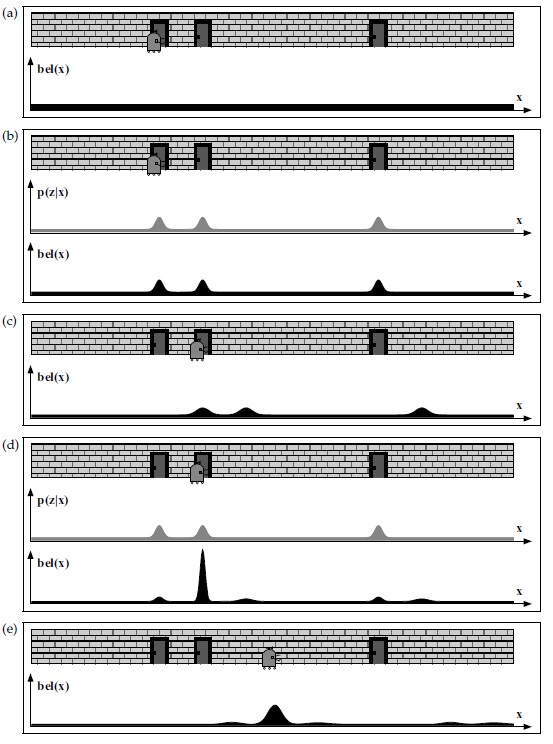
\includegraphics[width=1\linewidth]{11orig}}
	\caption{ (  Рис. 1.1 Общий принцип \textit{марковской локализации}: Мобильный робот в задаче глобальной локализации. Способы марковской локализации будут описаны в Главах 7 и 8.)}
	\label{fig:11orig}
\end{figure}
\begin{figure}
	\center{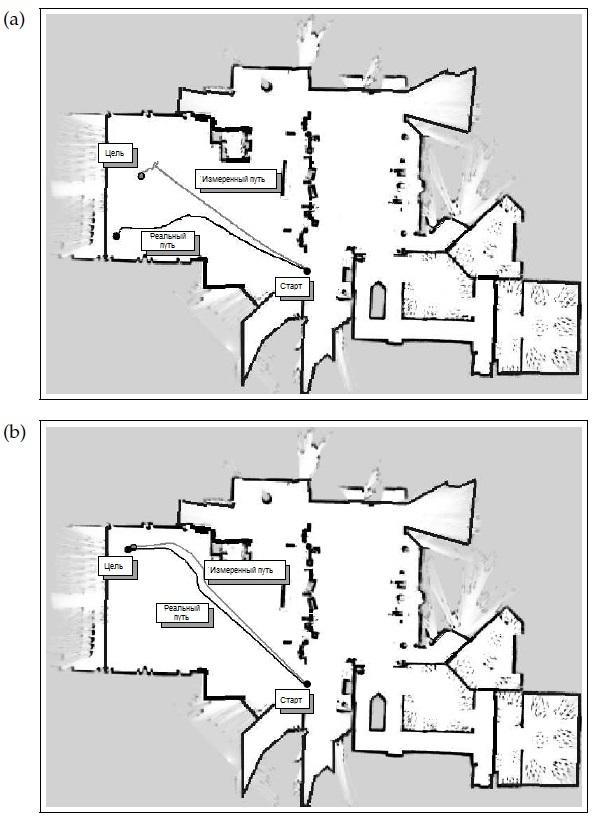
\includegraphics[width=1\linewidth]{12orig}}
	\caption{ ( Рис 1.2 Верхний рисунок: робот, который передвигается в открытом, безориентирном пространстве, может потерять возможность отслеживать своё местоположение. Нижний рисунок: Этого можно избежать, если оставаться около известных препятствий. Данные схемы иллюстрируют работу алгоритма, который называется  \textit{прибрежная навигация}, и будет обсуждаться в Главе 16. Рисунки являются собственностью Николаса Роя из MIT.)}
	\label{fig:12orig}
\end{figure}

Теперь допустим, что робот переместился. На схеме (c) Рис. 1.1 показан эффект воздействия движения на оценку роботом своего местоположения. Оценка была смещена в направлении движения.  Кроме того, ширина пиков увеличилась, отражая учёт дополнительной неопределённости, вызванной движением робота. На схеме (d) Рис. 1.1 показано оценочное распределение после обнаружения роботом ещё одной двери. Это следующее наблюдение заставило алгоритм разместить основную долю вероятности около одной из дверей, и робот, в данный момент, довольно уверенно оценивает своё местоположение. Наконец, на нижней схеме (e) показана оценка для случая, когда робот передвигается ещё дальше по коридору.

БАЙЕСОВСКИЙ ФИЛЬТР
 
Этот пример иллюстрирует многие аспекты вероятностной парадигмы. С точки зрения вероятности, проблему восприятия робота можно представить как задачу оценки состояния. Приведённый в примере локализации алгоритм известен как \textit{байесовский фильтр} и служит для нахождения апостериорной оценки в пространстве местоположений робота. Отображение информации представляет собой функцию плотности вероятности. Обновление функции отражает влияние дополнительной информации, полученной в результате измерений датчиков или же её потерю в силу влияния процессов окружающего мира, увеличивающих неопределённость.

ПРИБРЕЖНАЯ НАВИГАЦИЯ

Второй пример позволяет познакомиться с реалиями планирования и управления действиями робота. Как только что было сказано, с помощью вероятностных алгоритмов возможно вычислить степень неопределённости для робота в конкретный момент. Кроме этого, возможно учесть и будущую неопределённость, приняв ее во внимание при определении необходимых управляющих действий. Один из таких алгоритмов называется \textit{прибрежная навигация} \underline{("каботажная навигация"- прим. перев.)} и показан на Рис. 1.2. На рисунке изображена плоская карта реального здания. На верхней схеме показано сравнение реальной и расчётной траекторий. Наблюдаемое отклонение является результатом неопределённости для робота, которая только что обсуждалась. Представляет интерес факт того, что не все траектории подвержены одинаковой неопределённости. Траектория на Рис. 1.2a проходит по относительно открытому пространству, где почти нет ориентиров, которые робот может использовать, чтобы уточнить своё местоположение. На Рис. 1.2b показан альтернативный путь. В этом случае траектория сначала приближается к явно различимому с помощью датчиков углу, а затем проходит вблизи стены, что позволяет постоянно уточнять местоположения. Неудивительно, что неопределённость во втором случае существенно меньше, а это значит, что шансы действительно достичь расчётной целевой точки в конце маршрута заметно выше.

С помощью этой ситуации был проиллюстрирован лишь один из множества способов правильного учёта эффектов неопределённости в управлении роботом. В приведённом примере необходимость учёта возможной высокой неопределённости по одной из траекторий заставила робота предпочесть другой, более длинный путь, который позволил её уменьшить. Новый путь оказывается лучше в том смысле, что робот имеет гораздо более высокие шансы действительно оказаться у цели при достижении расчётной точки. Фактически, второй путь представляет иллюстрацию метода активного сбора информации. Робот, используя вероятностные соображения, определяет наилучший выбор действий таким образом, чтобы иметь возможность получать данные при продвижении к цели. Вероятностные способы планирования позволяют учесть неопределённость и запланировать сбор необходимой информации, а вероятностные способы управления – в полной мере использовать результаты такого планирования.\\

\textbf{1.3 Выводы}\\

Вероятностная робототехника органично объединяет в одно целое модели и данные датчиков, в то же время, обходя ограничения обоих. Эти принципы являются не просто прерогативой низкоуровневого управления, но проходят через все уровни программного обеспечения робота, от самых базовых до абстракций высшего уровня.

В отличие от традиционных подходов программирования в робототехнике — таких, как планирование движений на основе имитационной модели или реакции согласно шаблонам поведения, вероятностные методы обычно более надёжны в условиях наличия ограничений датчиков и моделей. Это позволяет гораздо легче, по сравнению с более старыми парадигмами, масштабировать их для сложных сред реального окружающего мира, где неопределённость  ещё более выражена. Де-факто, некоторые вероятностные алгоритмы являются единственным существующим рабочим решением для сложных проблем оценки ситуации в робототехнике, таких как проблема локализации, обсуждаемая чуть выше, или задача построения точных карт очень большого окружающего пространства.

По сравнению с традиционными подходами робототехники, полагающимися на модели, вероятностные алгоритмы менее требовательны к алгоритмам моделирования, что освобождает программиста от нелёгкой задачи улучшения их качества. Вдобавок, вероятностные алгоритмы ещё и не так чувствительны к точности датчиков робота, по сравнению с реактивными методами, для которых текущие показания датчиков являются единственным источником управляющего сигнала. С вероятностной точки зрения, \textit{проблема обучения робота} – всего лишь проблема оценки состояния в долгосрочной перспективе. Таким образом, вероятностные алгоритмы предоставляют чёткую методологию для многих аспектов обучения роботов.

Как всегда, наличие преимуществ имеет цену. Два наиболее часто упоминаемых ограничения вероятностных алгоритмов — \textit{вычислительная сложность} и использование \textit{приближенных вычислений}. Вероятностные алгоритмы изначально не так эффективны, как аналоги, не использующие вероятности. Это происходит потому, что вместо единственной аналитической оценки рассматриваются все плотности вероятности. Необходимость приближения возникает в силу  непрерывной природы большинства реальных сред, что значительно затрудняет получение точных апостериорных распределений. Правда, в некоторых редких случаях неопределённость удаётся довольно точно аппроксимировать, используя компактную параметрическую модель (например, нормальные распределения). Но чаще случается, что такие аппроксимации слишком неточны для практического использовать и необходимы более сложные представления.

Последние разработки в области аппаратного обеспечения позволили получить доступ к беспрецедентно высоким вычислительным мощностям по очень низкой цене, что положительно повлияло и на область вероятностной робототехники. Вдобавок, современные исследования позволили значительно повысить эффективность вероятностных алгоритмов для целого ряда сложных задач робототехники, многие из которых будут подробно рассмотрены в этой книге. Тем не менее,  вопрос вычислительной сложности остаётся, и мы ещё не раз подробно на нем остановимся, освещая сильные и слабые стороны конкретных вероятностных решений.\\

\textbf{1.4	Содержание}\\

Книга состоит из четырёх основных частей.\\

•	В Главах со второй по четвертую раскрываются общие математические принципы, лежащие в основе всех описанных в книге алгоритмов, а также некоторые ключевые алгоритмы. Материал этих глав составляет математическую основу всей книги.\\
 
•	В Главах 5 и 6 представлены вероятностные модели, используемые для мобильных роботов. Во многом, содержание этих главах представляет лишь вероятностное обобщение классических моделей робототехники. Эти алгоритмы образует робототехническую основу для изложения последующего материала.\\
 
•	Проблема локализации мобильного робота обсуждается в Главах 7 и 8. Здесь базовые оценочные алгоритмы объединяются с вероятностными моделями, обсуждаемыми в предыдущих двух главах.\\
 
•	Главы с 9 по 13 посвящены значительно более обширной проблеме составления карт местности для роботов. Как и ранее, они основываются на алгоритмах, описанных в начальных главах, дополненных новыми подходами, чтобы приспособить их к невероятной сложности задачи.\\
 
•	Вопросам планирования и управления с помощью вероятностных методов посвящены Главы с 14 по 17. Приведённые в начале раздела основные методы расширяются до практических алгоритмов вероятностного управления роботом. Завершающая Глава 17 посвящена обсуждению вероятностной точки зрения на проблему исследования с помощью роботов.\\

Книгу лучше всего читать в приведённом порядке, от начала до конца, хотя мы и постарались  каждую отдельную главу сделать самостоятельной и полной. Многочисленные разделы под названием \textit{“Математический вывод...”} при первом прочтении книги можно смело пропускать  без риска утратить целостность изложения и общее понимание материала.\\

\textbf{1.5 Обучение вероятностной робототехнике}\\

При использовании в качестве учебного пособия, мы \textit{не} рекомендуем преподавать главы в том порядке, в котором они приводятся в книге — если только студенты не отличаются необычайно сильной тягой к абстрактным математическим концепциям. Многочастичные фильтры легче объяснить, чем нормальные распределения, но студентам часто больше нравятся вопросы локализации мобильных роботов, нежели абстрактные алгоритмы фильтров. В наших курсах обучения мы обычно начинаем с Главы 2, а затем переходим прямо к Главам 7 и 8. Излагая вопросы локализации, по мере необходимости, мы возвращаемся к материалу в Главах с 3 по 7. Мы также рано преподаём материал Главы 14, чтобы как можно быстрее посвятить студентов в вопросы планирования и управления в рамках учебного курса.

В целях  преподавания Вы можете свободно использовать слайды и анимацию с веб-сайта книги\\
\hspace*{40mm} www.probabilistic-robotics.org \\
для иллюстрации различных алгоритмов. Также Вы можете послать нам, авторам, ссылки на веб-сайты Ваших учебных курсов и любой материал, который может быть полезен другим в процессе обучения Вероятностной Робототехнике.
 
Лучше всего изучать материал этой книги, имея возможность реализовать всё на практике. Нет ничего лучше для обучения робототехнике, чем программирование настоящего робота. Никто и ничто не может выявить трудности и подводные камни лучше, чем сама Природа!\\

\textbf{1.6 Библиографические примечания}\\

Робототехника, по мере развития, прошла долгий путь через целую серию принципов создания программного обеспечения. Первая парадигма сформировалась в середине 1970-х годов и известна как \textit{модельная парадигма}. Она началась с ряда исследований, продемонстрировавших трудности управления робототехническим манипулятором с большим количеством степеней свободы в непрерывных пространствах, в частности, с работы Рейфа (Reif, 1979). Позже она была в значительной степени развита в целом ряде публикаций, в частности, в аналитической работе Шварца (Schwartz et al., 1987) об оценке сложности движений робота. Канни (Canny, 1987) предложил первый полностью экспоненциальный алгоритм планирования движения, а Латомб (Latombe, 1991), опубликовал основополагающий текст о планировании движения на основе модели (многие другие ключевые достижения будут обсуждаться в Главе 14). В этих ранних работах проблема неопределённости, по большей части, игнорировалась, несмотря на уже начавшееся широкое использование рандомизации в качестве техники решения сложных проблем планирования движения (Кавраки с соавторами (Kavraki et al., 1996)). Напротив, неотъемлемым условием было наличие полной и точной модели робота, окружающей среды, а также полная определённость робототехнической системы. Модель при этом подразумевалась достаточно точной для обработки остаточной неопределённости с помощью одного лишь низкоуровневого контроллера движений. Большинство методов планирования движения просто создавало единичную эталонную траекторию для управления манипулятором, хотя методы \textit{потенциальных полей} (Хатиб (Khatib, 1986) и \textit{навигационных функций} (Кодишек (Koditschek, 1987) и предоставляли механизмы реагирования на непредвиденные факторы. Реализации этих ранних методов, если таковые вообще имелись, были ограничены искусственными средами, где любые проявления неопределённости могли быть устранены механическими методами или же с достаточной точностью измерены.
 
Ситуация радикально изменилась в середине 1980-х, когда все исследовательское сообщество робототехники обратило пристальное внимание на проблему недостатка обратной связи от датчиков. С большой уверенностью  для области \textit{поведенческой робототехники} была отвергнута идея необходимости наличия любой внутренней модели. Вместо этого было введён принцип взаимодействия \textit{ситуационного агента} с физической средой (Кэлблинг и Розеншайн (Kaelbling и Rosenschein) 1991), что  придало движениям робота комплексный характер (феномен, часто называемый \textit{непредсказуемым поведением} (Стилз (Steels, 1991)). Теперь уже определяющую роль играло сенсорное обнаружение, и внутренние модели были отвергнуты (Брукс (Brooks) 1990).

Энтузиазм на поприще поведенческой парадигмы подогревался ранними успехами, когда удалось далеко превзойти возможности традиционных алгоритмов планирования движения на основе моделей. Одним из первых успешных образцов стал “Чингиз” ("Genghis"), шестиногий робот, разработанный Бруксом (Brooks, 1986). Относительно простой алгоритм на основе конечного автомата оказался способен управлять передвижением робота даже по пересечённой местности. Ключ к успеху данного метода состоял в сенсорном восприятии: управление было полностью определено характеристиками взаимодействия с окружающей средой, воспринимаемой с помощью датчиков робота. На основе некоторых ранних работ был создан достаточно сложный робот, использующий комплексную обратную связь от окружающей среды (Коннелл (Connell, 1990)). Позже эта подход стал коммерчески успешным в виде проекта робота-пылесоса (IRobots Inc., 2004), программное обеспечение которого также было построено на основе поведенческого подхода.

В силу малого количества внутренних моделей и особого внимания к простым механизмам управления, большинство робототехнических систем были ограничены относительно несложными задачами, в которых текущих данных с датчиков было достаточно для выбора верного варианта управления. Чтобы обойти это ограничение, в более современных работы используются архитектуры \textit{гибридного управления} (Аркин (Arkin, 1998)), когда низкоуровневое управление обеспечивается поведенческими методами, а планировщик на основе модели координирует действия робота на высоком, абстрактном уровне. Такие гибридные архитектуры получили широкое распространение в сегодняшней робототехнике. Они хорошо согласуются с фундаментальной работой по трехуровневым архитектурам, написанной Гэтом (Gat, 1998), начало которой было положено «Роботом Шейки» Нилссона ("Shakey the Robot", Nilsson 1984).

С середины 1990-х вероятностная робототехника пережила этап развития , хотя ее базовые принципы можно проследить вплоть до изобретения калмановского фильтра (Kalman, 1960). Во многом, она занимает промежуточное место между модельными и поведенческими методами. В вероятностной робототехнике имеются модели, но считается, что они неполны и недостаточны для осуществления управления. Принимаются во внимание и показания датчиков, но и они не считаются достаточными. Действие управления может быть определено путём комбинирования обеих составляющих – модели и данных измерений датчиков.  Для интеграции моделей и измерений датчиков в одно целое используются математические методы статистики.

Многие из ключевых достижений в области вероятностной робототехники будут обсуждаться в будущих главах. Некоторые из фундаментальных открытий в этой области включают изобретение Смитом и Чизманом (Smith и Cheeseman, 1986) методов калмановской фильтрации для решения проблем восприятия в большом количестве измерений, открытие карт сеток занятости (Элфис (Elfes), 1987, Моравиц (Moravec), 1988), и вторичное введение в обиход  методов планирования при неполной информации наблюдений Кэлблингом с соавторами (Kaelbling et al., 1998). В последнее десятилетие наблюдалось просто прорывное развитие новых методов: широкую популярность приобрели многочастичные фильтры (Деллаэрт с соавторами (Dellaert et al.), 1999), были разработаны новые методологии программирования на основе байесовских методов обработки информации (Трун (Thrun), 2000, Лебелтел с соавторами (Lebeltel et al.) 2004, Парк с соавторами (Park et al.), 2005). Это развитие происходило рука об руку с созданием физических робототехнических систем под управлением вероятностных алгоритмов, таких, как промышленные механизмы для перемещения грузов, описанные в работе Дюрран-Уайта (Durrant-Whyte, 1996), развлекательных роботов для музеев (Баргард (Burgard et al.), 1999, Трун (Thrun et al.), 2000, Зигварт (Siegwart et al.), 2003), и роботов медицинского назначения, приспособленных для ухода за больными (Пино (Pineau et al.), 2003). Программный пакет управления мобильным роботом с открытым исходным кодом  и широким использованием вероятностных методов был представлен в работах Монтемерло с соавторами (Montemerlo et al., 2003a).

Отрасль коммерческой робототехники также подошла к поворотной точке. В ежегодном Мировом обзоре робототехники (World Robotics Survey), опубликованном Европейской комиссией ООН и \textit{Международной федерацией робототехники} в 2004 году был отмечен годовой прирост мирового рынка робототехники на 19\%. Ещё более примечателен факт изменения структуры рынка, указывающий на переход от промышленного использования к сервисным роботам и потребительским продуктам.\\
 
\textbf{\Large2 Рекурсивная оценка состояния}\\

\textbf{2.1 Введение}\\

Ключевая идея вероятностной робототехники состоит в оценке состояния на основе информации от датчиков. Эта задача сводится к оценке численных показателей, которые напрямую измерить невозможно, но можно каким-то образом воспринять их из свойств внешнего мира. 
В большинстве приложений робототехники довольно просто определить, что же нужно делать, если известны \textit{точные} значения параметров. Например, перемещать мобильного робота, если известны точные местоположения как самого робота, так и всех ближайших препятствий, довольно легко. К сожалению, напрямую измерить эти значения невозможно и для получения нужной информации робот вынужден полагаться на измерения датчиков,  способные передать только частичную информацию, при этом часто  повреждённую воздействием помех.  Оценка состояний производится для того, чтобы попытаться восстановить состояние переменной на основе имеющихся данных. Вероятностные алгоритмы оценки состояния вычисляют распределения оценок по всем возможным состояниям. Пример вероятностной оценки состояний  уже приводился во вводной части книги – это проблема локализации мобильного робота.
 
Целью этой главы является представление базовой системы понятий и математических инструментов для оценки состояния на основе данных датчиков.

• В подразделе 2.2 вводятся основные концепции теории вероятности, использованные в книге.
 
• В подразделе 2.3 описывается формальная модель взаимодействия робота с окружающей средой и вводится ключевая терминология, которая используется в книге.
 
• В подразделе 2.4 впервые описываются \textit{байесовские фильтры}, рекурсивный алгоритм оценки состояния, образующий первооснову для практически каждого представленного метода.
 
• В подразделе 2.5 обсуждаются трудности представлений и вычислений, которые возникают при использовании байесовских фильтров.\\

\textbf{2.2 Основные концепции теории вероятности}\\

Этот подраздел знакомит читателя с основными обозначениями и фактами теории вероятности, которые используются в книге. 
В вероятностной робототехнике все величины, такие как измерения датчиков, управляющие воздействия, состояние робота и окружающей среды, смоделированы с помощью случайных переменных.

СЛУЧАЙНЫЕ ПЕРЕМЕННЫЕ

\textit{Случайные переменные} способны принимать несколько значений в соответствии с определёнными правилами теории вероятности. 
Вероятностное заключение – это процесс вычисления таких правил для случайных величин, зависящих от других случайных величин и наблюдений.
 
Обозначим через $X$ случайную переменную, а $x$ – конкретное значение, которое может принимать $X$. Стандартным примером случайной переменной является исход \textit{броска монеты}, где $X$ может принимать значения \textit{«орла}» или \textit{«решки»}. Если пространство всех значений, которые способна принимать $X$, дискретно, как в случае броска монеты, то можно записать\\

(2.1) $$p(X = x)$$\\
чтобы обозначить вероятность того, что случайная переменная  $X$ принимает значение $x$. Например, для «честной» монеты эта величина характеризуется как $p(X$ = «орёл») = $p(X$ = «решка») = 1/2. Сумма всех дискретных вероятностей равна единице, отсюда \\

(2.2) $$\sum_{x}p(X = x) = 1$$\\
Вероятности также всегда неотрицательны, поэтому $p(X = x)\ge0$.

Для упрощения записи обычно будем опускать точное указание случайной переменной и использовать сокращение $p(x)$ вместо того, чтобы писать $p(X = x)$.

Большинство методов в этой книге имеет дело с оценкой и процессом принятия решений в непрерывных пространствах. Непрерывные пространства характеризуются тем, что случайные переменные способны принимать значения из непрерывного диапазона.
Если иное не указано специально, будем считать, что\\
ПЛОТНОСТЬ ВЕРОЯТНОСТИ\\ 
все непрерывные случайные переменные имеют \textit{функции плотности вероятности} (ФПВ - PDF). Обычно функция плотности представляет собой одномерное \textit{нормальное распределение}\\
НОРМАЛЬНОЕ РАСПРЕДЕЛЕНИЕ\\ 
с математическим ожиданием $\mu$ и среднеквадратичным отклонением $\sigma^2$. ФПВ нормального распределения\\
ГАУССИАН\\ 
выражена следующей \textit{функций Гаусса}:\\

(2.3)
 $$p(x)=(2\pi\sigma^2)^-{}^\frac{1}{2}exp\left\lbrace -\frac{1}{2}\frac{(x-\mu)^2}{\sigma^2}\right\rbrace $$
Нормальные распределения играют важную роль в книге. Часто мы будем сокращать их до 
$N(x;\mu,\sigma^2)$, что означает случайную переменную, её математическое ожидание и среднеквадратичное отклонение.
 
Для нормального распределения (2.3)  $x$ считается скалярным значением. Однако, часто $x$ будет представлен в виде многомерного вектора. Нормальные распределения векторов называются \textit{многомерными}.\\
МНОГОМЕРНОЕ РАСПРЕДЕЛЕНИЕ\\
Многомерные нормальные распределения характеризуются функциями распределения вероятности следующего вида:\\
 
(2.4)$$p(x)=det(2\pi\varSigma)^-{}^\frac{1}{2}exp\left\lbrace -\frac{1}{2}(x-\mu)^T\varSigma^-{}^1(x-\mu)\right\rbrace $$
 Здесь $\mu$ - многомерный вектор, а $\varSigma$ - \textit{неотрицательно определённая симметричная} матрица, называемая \textit{ковариационной}\\
 КОВАРИАЦИОННАЯ МАТРИЦА\\
 Верхний индекс $T$ означает транспонирование вектора. Аргумент экспоненты в функции квадратичен по $x$, с параметрами квадратичной функции $\mu$ и $\varSigma$.
 
 Следует обратить внимание, что Выражение (2.4) является строгим обобщением Выражения (2.3). Оба уравнения равны, если  $x$ - скалярное значение, а $\varSigma=\sigma^2$.
 
 Уравнения (2.3) и (2.4) – это примеры функций распределения вероятности. Точно так же, как сумма дискретного распределения вероятности равна 1, интеграл ФПВ всегда равен единице:\\

 (2.5) $$\int p(x) dx = 1$$
 Однако, в отличие от дискретной вероятности, значения ФПВ не ограничены сверху единицей. В ходе изложения в этой книге понятия \textit{вероятности, плотности вероятности} и \textit{функции плотности вероятности} будет использоваться как взаимозаменяемые. По умолчанию будем  считать, что все непрерывные случайные переменные измеримы, а также, что для всех непрерывных распределений существуют плотности вероятности.\\ 
 СОВМЕСТНОЕ РАСПРЕДЕЛЕНИЕ\\
 
 \textit{Совместное распределение} двух случайных переменных $X$ и $Y$ выражается в виде\\

 (2.6) $$p(x, y) = p(X = x ; Y = y)$$
 Это выражение описывает вероятность  события, когда случайная переменная $X$ принимает значение $x$, и одновременно, переменная $Y$  принимает значение $y$. Если $X$ и $Y$ \textit{независимы},\\
 НЕЗАВИСИМОСТЬ\\
 то получится, что\\

 (2.7) $$p(x, y) = p(x) p(y)$$
 Часто случайные переменные уже содержат определённую информацию о других случайных переменных.
 Допустим, уже известно, что значение $Y$  равно $y$, и хотелось бы узнать вероятность того, как значение $x$  переменной $X$ связано с этим фактом. Такая вероятность будет равна\\

 (2.8) $$p(x | y) = p(X = x | Y = y)$$ 
 УСЛОВНАЯ ВЕРОЯТНОСТЬ\\
 и называться \textit{условной вероятностью}. При $p(y) > 0$ условная вероятность определяется как\\ 

 (2.9) $$p(x | y) = \frac{p(x,y)}{p(y)}$$
 Если $X$ и $Y$ независимы, то получится, что\\

 (2.10) $$p(x | y) = \frac{p(x)p(y)}{p(y)}=p(x)$$ 
 Другими словами, при независимости $X$ и $Y$, информация о значении $Y$ никак не поможет узнать значение $X$. Независимость и ее обобщение, известное как условная независимость играют очень важную роль в этой книге.
 
 Интересный факт, который является следствием определения условной вероятности\\ 
 ТЕОРЕМА О ПОЛНОЙ ВЕРОЯТНОСТИ\\
 и аксиом мер вероятности, часто называют \textit{Теоремой о полной вероятности}:\\
 
 (2.11) $$p(x)=\sum_y p(x | y) p(y) \qquad\mbox {(для дискретного случая)}$$
 
 (2.12) $$p(x)=\int p(x | y) p(y)dy \qquad\mbox {(для непрерывного случая)}$$
 Если $p(x | y)$ или $p(y)$ равны нулю, можно и произведение   $p(x | y)$ $p(y)$ принять равным нулю, вне зависимости от оставшегося множества.\\
 ТЕОРЕМА БАЙЕСА\\
 
 Также очень важна \textit{теорема Байеса}, которая определяет отношение вероятности $p(x | y)$ к его «противоположности» $p(y | x)$. Для теоремы требуется, чтобы $p(y) > 0$:\\

 (2.13) $$p(x | y)=\frac{p(y | x) p(x)}{p(y)}=\frac{p(y | x) p(x)}{\varSigma_{x'}p(y | x') p(x')}\qquad\mbox {(дискретный случай)}$$
 
 (2.14) $$p(x | y)=\frac{p(y | x) p(x)}{p(y)}=\frac{p(y | x) p(x)}{\int p(y | x') p(x')dx'}\qquad\mbox {(непрерывный случай)}$$
 
 Теорема Байеса играет определяющую роль в вероятностной робототехнике (как и вообще в вероятностных выводах). Если $x$  - это количество, которое бы нам хотелось узнать на основании $y$,\\
 АПРИОРНАЯ ВЕРОЯТНОСТЬ\\
 то вероятность $p(x)$ будет называться \textit{априорным распределением вероятности}, а $y$ будет называться \textit{данными} (например, измерений датчиков). В распределении $p(x)$ суммируются все данные, имеющиеся об $X$, без учёта $y$.\\
 АПОСТЕРИОРНАЯ ВЕРОЯТНОСТЬ\\
 Вероятность $p(x | y)$ называется \textit{апостериорным распределением вероятности} по $X$.
 В силу Выражения (2.14), теорема Байеса даёт удобный способ вычислить апостериорную вероятность $p(x | y)$ на основе «перевёрнутой» условной вероятности $p(y | x)$ и априорной вероятности $p(x)$. Другими словами, если необходимо получить значение $x$ на основе данных датчиков $y$, теорема Байеса позволяет сделать это с помощью обратной вероятности, определяющей значение $y$ при условии, что имело место событие $x$.\\
 ПОРОЖДАЮЩАЯ МОДЕЛЬ\\
 В робототехнике вероятность $p(y | x)$ часто называют \textit{порождающей моделью}, поскольку она, на некотором уровне абстракции, описывает, каким образом переменные состояния $X$ \textit{становятся причиной} изменения показаний датчиков $Y$.
 
 Важно отметить, что знаменатель $p(y)$ в теореме Байеса не зависит от $x$. Таким образом, множитель $p(y)^{-1}$ в уравнениях (2.13) и (2.14) будет одинаковым при любом значении $x$ апостериорной вероятности $p(x | y)$. В силу этого, $p(y)^{-1}$ часто именуют  \textit{нормирующим членом} в теореме Байеса и, в общем виде, записывают как $\eta$:\\

 (2.15) $$p(x | y)=\eta p(y | x) p(x)$$
 Преимуществом такой записи является ее лаконичность. Вместо явной записи точной формулы нормирующей константы (а она может вырасти до весьма больших размеров в некоторых математических выводах), просто запишем символ нормировки $ \eta $, чтобы показать, что конечный результат должен быть нормирован до единицы. В этой книге подобные нормировщики будут записываться как $\eta$(или $\eta', \eta''$, . . . ). 
 \textbf{Важно:} Мы будем произвольно использовать в различных равенствах одно и то же обозначение нормирующего члена $ \eta $, даже если его реальное значение различается.
 
 Заметим, что будет совершенно справедливым переписать любую из обсуждаемых теорем, используя произвольные случайные переменные, скажем, переменную $ Z $. Например,  запись теоремы Байеса, при $Z = z$, даст следующее равенство:\\

 (2.16)$$p(x | y, z) = \frac{p(y | x, z) p(x | z)}{p(y | z)}$$
 пока  $p(y | z) > 0$.
 
 Аналогично, можем переписать правило для комбинирования вероятностей независимых случайных переменных (2.7), используя переменную $z$:\\
 
 (2.17) $$p(x, y | z) = p(x | z) p(y | z)$$
 
 УСЛОВНАЯ НЕЗАВИСИМОСТЬ\\
 Такое отношение называется \textit{условной независимостью}. Читатель может легко убедиться, что (2.17) эквивалентно\\

 (2.18) $$p(x | z) = p(x | z, y)$$
 
 (2.19) $$p(y | z) = p(y | z, x)$$\\
 Условная независимость играет важную роль в вероятностной робототехнике. Она применяется, когда переменная $y$ не несёт никакой информации о переменной $x$, при условии, что известно значение другой переменной $z$. Условная независимость не предполагает (абсолютной) независимости, а значит\\
 
 (2.20) $$p(x, y | z) = p(x | z) p(y | z) \nRightarrow p(x, y) = p(x) p(y)$$
 Обратное также, в общем случае, неверно, поскольку абсолютная независимость не предполагает условной независимости:\\
 
 (2.21) $$p(x, y) = p(x) p(y) \nRightarrow p(x, y | z) = p(x | z) p(y | z)$$
 В отдельных случаях условная и абсолютная независимость могут совпадать.
  
 В ряде вероятностных алгоритмов требуется вычислять признаки или статистики вероятностных распределений.\\ 
 МАТЕМАТИЧЕСКОЕ ОЖИДАНИЕ СЛУЧАЙНОЙ ПЕРЕМЕННОЙ\\
  \textit{Математическое ожидание} случайной величины $X$ обозначается как\\
 
 (2.22) $$E[X] =\sum_{x}x p(x)\qquad\mbox {(дискретный случай)}$$
  
 (2.23) $$E[X] = \int x p(x) dx\qquad\mbox {(непрерывный случай)}$$ 
 Некоторые случайные переменные не имеют конечного математического ожидания, однако, такие исключения в материале книги рассматриваться не будут.
 
 Математическое ожидание – это линейная функция случайной переменной. В частности, можно записать\\
 
 (2.24) $$E[aX + b] = aE[X] + b$$
 для произвольных числовых значений $a$ и $b$. Ковариация $X$ получается следующим образом\\

 (2.25) $$Cov[X] = E[X-E[X]]^2=E[X^2]-E[X]^2$$
 Ковариация означает квадрат ожидаемого отклонения от значения математического ожидания. Как было указано ранее, математическое ожидание многомерного нормального распределения $N (x; \mu, \varSigma)$ равно $ \mu $, тогда  его ковариация будет  $ \varSigma $.\\
 ЭНТРОПИЯ
 
 Последней важной концепцией этой книги является \textit{энтропия}. Энтропия вероятностного распределения задаётся следующим выражением:\\

 (2.26) $$H_p(x) =E[-\log_2p(x)]$$
 которое можно выразить в следующем виде\\
 
 (2.27) $$H_p(x)=-\sum_{x}p(x) \log_2 p(x)\qquad\mbox {(дискретный случай)}$$ 

 (2.28) $$H_p(x) ={-}\int p(x) \log_2 p(x) dx\qquad\mbox {(непрерывный случай)}$$
 {}\\
 \begin{figure}[h]
 	\center{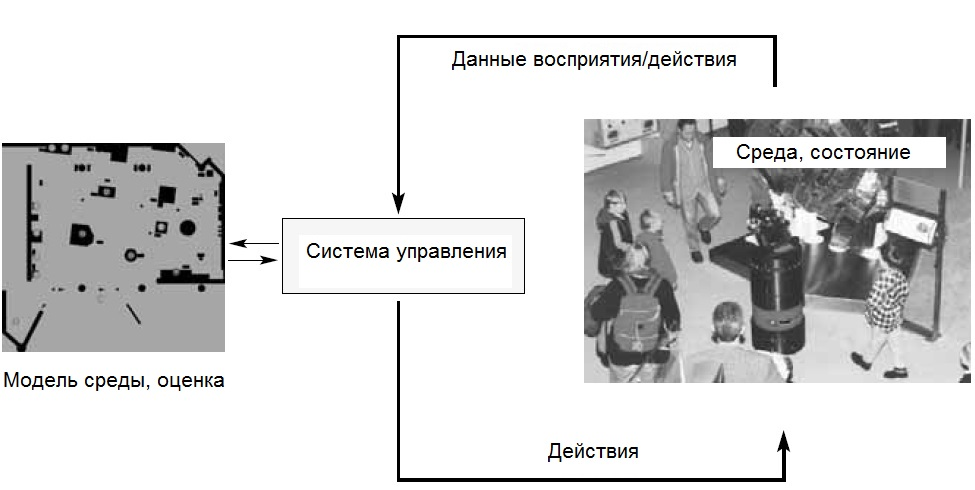
\includegraphics[width=0.8\linewidth]{21orig}}
 	\caption{ Рис.2.1. Взаимодействие робота с окружающей средой.}
 	\label{fig:21orig}
 \end{figure}
 

 Концепция энтропии происходит из теории информации. Энтропия- это ожидаемое количество информации, которое содержит значение $x$. В дискретном случае, для
 ${-}\log_2 p(x)$ означает количество бит, требуемое для кодирования $x$ оптимальным образом, подразумевая, что $p(x)$ – вероятность появления значения $x$. В данной книге понятие энтропии будет использовано в контексте сбора информации роботом, выражая, таким образом, количество информации, которую робот может получить, совершая определённые действия.\\ 
 
\textbf{ 2.3 Взаимодействие робота с окружающей средой}

 На Рис. 2.1 показано взаимодействие робота с окружающей средой.\\ 
 ОКРУЖАЮЩАЯ СРЕДА РОБОТА\\
 \textit{Окружающая среда} или \textit{«мир»} - это динамическая система, обладающая внутренним состоянием.
 Робот способен получать информацию об окружающем мире, используя датчики. 
 Но с датчиков поступает зашумленный сигнал, и, вдобавок, имеется множество факторов, которые невозможно измерить напрямую. 
 Как следствие, робот формулирует некое внутреннее суждение относительно состояния окружающей среды на основании собранных и имеющихся данных, что показано слева на схеме.
  
 Робот также способен воздействовать на окружающую среду с помощью приводов. Эффект таких действий очень часто несёт некоторую непредсказуемость, поэтому каждое действие управления влияет как на состояние окружающей среды, так и на внутреннее представление этого состояния роботом.
  
 Опишем это взаимодействие более формально.\\
 
 \textbf{2.3.1 Состояние}\\
 
 СОСТОЯНИЕ
 
 Окружающая среда характеризуется \textit{состоянием}. В материале, представленном в книге, удобно понимать термин «состояние» как обозначение набора всех отличительных черт робота и его окружения, способных повлиять на будущее. Некоторые переменные состояния изменяются со временем, например, местонахождение людей в непосредственной близости от робота. Другие остаются постоянными, такие, как расположение стен в большинстве зданий.
 Изменяющиеся состояния назовём \textit{динамическими}, чтобы отличать их от \textit{статических}, то есть неизменных, состояний. Состояние также включает переменные, описывающие самого робота, такие как его положение, скорость, исправность датчиков и так далее.
  
 В книге состояние будет обозначено $x$, несмотря на то, что конкретные переменные, включённые в $x$, могут различаться, в зависимости от контекста. Состояние в момент времени $t$ будет обозначаться как $x_t$. В книге используются следующие типичные переменные состояния:\\
 
 ПОЛОЖЕНИЕ\\
 • \textit{Положение} робота, определяет его местоположение и ориентацию в пространстве относительно глобальной координатной сетки.
 Мобильные роботы жёсткой конструкции имеют шесть переменных состояния, три, обозначающие координаты в прямоугольной системе, и три - для углов положения в пространстве (крен, тангаж, рысканье). Для мобильных роботов, действующих в плоских окружающих средах, положение обычно задаётся тремя переменными - двумя координатами на плоскости и углом направления движения (рысканье).\\
 
 • При управлении роботом описание его положения включает переменные для \textit{конфигурации приводов}. Это могут быть, например, углы поворота для вращающихся сочленений. 
 Каждая степень свободы  манипулятора робота характеризуется одномерной конфигурацией в произвольный момент времени и является составляющей кинематического состояния робота. Конфигурация робота часто обозначается как \textit{кинематическое состояние}.\\
  
 • \textit{Скорость робота} и \textit{скорости сочленений} обычно обозначаются как \textit{динамическое состояние}. Для робота жёсткой конструкции, передвигающегося в пространстве, можно вывести до шести переменных скорости, по одной для каждого направления перемещения.  Динамическое состояние играет очень небольшую роль в книге.\\
 
 • \textit{Местоположение и признаки объектов окружающего  мира} также являются переменными состояния. Объектом может быть дерево, стена или даже пиксель на более обширной поверхности, а их характеристикой, например, внешний вид (цвет, текстура). В зависимости от степени детализации моделируемого состояния, описание окружающей среды может иметь от нескольких десятков до сотен миллионов переменных состояния (или даже больше). Только представьте, сколько бит потребуется для точного описания вашего окружения! Для многих задач, обсуждаемых в книге, местоположение объектов в окружающей будет неизменным.\\
 ОРИЕНТИР \\
 Для некоторых задач объекты могут считаться разновидностью \textit{ориентиров}, которые представляют собой хорошо различимые, стационарные признаки окружающей среды, которые можно надёжно распознать.\\
  
 • \textit{Местоположение и скорости движущихся объектов и людей} также являются потенциальными переменными состояния. Часто робот является не единственным движущимся объектом в окружающей среде. Для других движущихся сущностей выделяются собственные наборы из кинематического и динамического состояний.\\
 
 • Существует множество других переменных состояния, которые могут повлиять на ориентацию робота в пространстве. Например, переменной состояния может стать факт исправности датчика, или же уровень заряда для робота, работающего от аккумуляторов. Список потенциальных переменных состояния бесконечен!\\
 
 ПОЛНОЕ СОСТОЯНИЕ
  
 Состояние $x_t$ назовём \textit{полным}, если оно наилучшим образом может быть использовано для предсказания будущего состояния. Другими словами, "полнота" означает, что знание прошлых состояний, измерений или управляющих действий не даёт дополнительной информации, которая могла бы помочь ещё более точно предсказать будущие изменения. Важно заметить, что наше определение полноты не требует того, чтобы будущее было \textit{детерминированной} функцией состояния. 
 Оно может быть и стохастическим, но никакие переменные, кроме $x_t$, не могут повлиять на стохастическое развитие будущих состояний, если только эта зависимость не управляется  состоянием $x_t$.\\
 МАРКОВСКИЕ ЦЕПИ\\
 Временные процессы, отвечающие этим условиям, широко известны под названием \textit{марковских цепей}.
 
 Категория полноты состояния, в основном, имеет лишь теоретическую важность. На практике невозможно определить полное состояние для любой реалистичной робототехнической системы. По настоящему "полное" состояние будет включать не только все аспекты окружающего, которые могут повлиять на будущее, но также и самого робота, содержимое памяти его компьютера, образы мозга окружающих людей, и так далее. Некоторые из этих данных довольно трудно получить, поэтому практические реализации ограничены лишь небольшим набором из всех возможных переменных состояния.\\
 НЕПОЛНОЕ СОСТОЯНИЕ\\ 
 Такое состояние называется \textit{неполным}.
  
 В большинстве задач практического использования роботов состояние $x_t$ непрерывно и определено на непрерывном множестве. Хорошим примером непрерывного пространства состояний является положение робота, представляющее совокупность местоположения и ориентации во внешней системе координат. Иногда, впрочем, состояние дискретно. Примером дискретного пространства состояний является, скажем, бинарная переменная состояния, моделирующая факт исправности датчика. Пространства состояний, которые содержат как непрерывные, так и дискретные переменные, называются \textit{гибридными}.
 
 В большинстве интересующих нас задач робототехники пространство изменяются со временем. В данной книге время будет считаться дискретным. Это означает, что все интересующие нас события произойдут в конкретные моменты времени $t = 0, 1, 2 . . .$. Если робот начинает функционировать в определённый момент времени, будем считать, что  для этого момента $t = 0$.\\
 
 \textbf{2.3.2 Взаимодействие со средой}\\
 
 Есть два основных типа взаимодействия между роботом и средой: робот может изменять состояние своего окружения с помощью приводов и собирать информацию об этом состоянии с помощью датчиков. 
 Оба типа взаимодействия могут происходить одновременно, но, для удобства изложения, в книге они будут разделены. Взаимодействие показано на Рис. 2.1.\\
 
 • \textbf{Измерение параметров окружающей среды датчиками}. Восприятие - это процесс получения данных о состоянии окружающей среды с помощью датчиков робота. Например, в целях получения необходимых данных, можно принимать изображение с камеры, определить дальность до препятствия, использовать тактильные датчики и так далее.\\
 ИЗМЕРЕНИЕ\\
 Результат такого взаимодействия в целях восприятия будем называть \textit{измерением}, хотя иногда будут использоваться такие термины, как \textit{наблюдение} или \textit{представление}. Обычно, информация измерений поступает с некоторой задержкой, и описывает состояние, которое было несколько мгновений назад.\\
 
 • \textbf{Действия управления} изменяют состояние окружающего мира с помощью приложения сил к предметам окружающей среды.\\УПРАВЛЯЮЩЕЕ ДЕЙСТВИЕ\\ Примеры \textit{управляющих действий} включают движение робота и манипулирование объектами. Даже если робот не выполняет никаких действий, состояние обычно изменяется. Поэтому, для сохранения целостности изложения, будем считать, что робот \textit{всегда} выполняет управляющее действие вне зависимости от того, было ли принято решение перемещать какой-либо из приводов.
 На практике, робот непрерывно и одновременно выполняет управляющие действия и измерения.\\
  
 Теоретически, робот может сохранять записи всех прошлых измерений и управляющих действий. Условимся называть такую совокупность информации \textit{данными} (вне зависимости от того, были ли они сохранены). Поскольку выполняется два типа взаимодействий с окружающей средой, робот имеет доступ к двум разным потокам данных.\\
 
 • \textbf{Данные измерений параметров окружающей среды} предоставляют информацию о текущем состоянии окружения. Примерами данных измерений служат изображение с камеры, определение расстояния и так далее. В большинстве разделов книги мы будем просто игнорировать малые эффекты запаздывания (например, большинство лазерных датчиков последовательно сканируют окружающее пространство c очень высокой скоростью, но мы просто будем считать, что имеется измерение, относящееся к конкретному моменту времени). Данные измерений в момент времени $t$ будет обозначаться как $z_t$.\\ 
 При изложении будем просто считать, что робот выполняет единственное измерение в один момент времени. Это допущение служит, в основном, для удобства обозначения, поскольку почти все алгоритмы книги могут быть легко расширены для роботов, которые получают произвольное число измерений в течение одного такта времени. Запись\\  

 (2.29)$$z_{t_1:t_2}=z_{t_1},z_{t_1+1},z_{t_1+2},...,z_{t_2}$$ 
 обозначает набор всех переменных, полученных с момента времени $t_1$ до $t_2$, при этом $t_1\leq t_2$.\\
 
 • \textbf{Данные управления} содержат информацию об \textit{изменении состояния} в окружающей среде. В мобильной робототехнике типичным примером данных управления является скорость робота. Установка значения скорости 10 см в секунду в течение пяти секунд предполагает, что после выполнения команды на движение робот переместится в положение, находящееся, приблизительно, на 50 см впереди от начального. Таким образом, сигнал управления передаёт информацию об изменении состояния.\\
 ОДОМЕТР\\
 Дополнительным источником данных управления являются \textit{одометры} – датчики, которые измеряют количество оборотов колес робота и, таким образом, передают информацию об изменении состояния. Хотя, строго говоря, одометры – это датчики, условимся считать показания одометра данными управления, поскольку с их помощью измеряется эффект управляющего действия.\\
 Данные управления будут обозначаться как $u_t$. Переменная $u_t$ будет всегда связана с изменением состояния в интервале времени $\left( t-1;t\right] $. Как и ранее, обозначим последовательности данных управления через $u_{t_1:t_2}$, для $t1\leq t2$:\\

 (2.30) $$u_{t_1:t_2} = u_{t_1},u_{t_1+1},u_{t_1+2}, . . . , u_{t2}$$
 Поскольку состояние среды может изменяться, даже если робот не выполняет никакого определённого действия, то, технически говоря, сам факт изменения времени содержит информацию об управлении. В силу этого, условимся, что каждый такт времени $t$ происходит ровно одно действие управления, при этом возможно действие \textit{«не делать ничего»}.\\ 
 
 Разница между измерением и управлением критически важна, поскольку в материале, который будет излагаться, оба типа данных играют фундаментально различные роли. Восприятие окружающей среды предоставляет дополнительную информацию о её состоянии, и, таким образом, увеличивает осведомлённость робота. Движение, с другой стороны, часто приводит к потере информации из-за наличия собственных шумов приводов и случайных факторов окружающей среды. Такое разделение ни в коей мере не предполагает разделения во времени восприятия и действий. Восприятие и управление осуществляются одновременно, а их разделение преследует лишь цели удобства изложения.\\
 
 \textbf{ 2.3.3 Вероятностные генеративные правила}\\
 
 Процесс изменения состояний и измерений управляется правилами теории вероятности. В общем случае, состояние $x_t$ стохастически возникает из состояния $x_{t-1}$. В силу этого, имеет смысл определить вероятностное распределение, из которого было сгенерировано $x_t$.
 На первый взгляд, появление состояния $x_t$ может быть обусловлено всеми предыдущими состояниями, измерениями и действиями управления. Следовательно, вероятностные правила, характеризующие эволюцию состояния, могут быть изложены в виде вероятностного распределения следующего вида:
 $p(x_t | x_{0:t-1}, z_{1:t-1}, u_{1:t})$. Обратите внимание, что нет никакой причины считать, что робот сначала совершает действие управления $u_1$, а после этого – производит измерение $z_1$.
 
 Важным является следующее суждение: Если состояние $x$ полное, значит в нём в достаточной степени суммируется всё произошедшее на предыдущих тактах времени. В частности, $x_{t-1}$ является достаточной статистической величиной для всех предыдущих действий управления и измерений вплоть до указанного момента времени, 
 $u_{1:t-1}$ и $z_{1:t-1}$, соответственно. Из всех переменных, приведённых выше, если известно состояние $x_{t-1}$, только управление $u_t$ будет иметь значение.
 
 В терминах теории вероятности, это рассуждение можно выразить следующим равенством:\\
 
 (2.31) $$p(x_t | x_{0:t-1}, z_{1:t-1}, u_{1:t}) = p(x_t | x_{t-1}, u_t)$$
 Выраженное этим равенством свойство является примером \textit{условной независимости}. Утверждается, что некоторые переменные независимы от других, если известны значения третьей группы переменных, называемых условными переменными. Условная независимость будет широко использована в книге, поскольку она является главным фактором вычислительной разрешимости большинства приведённых алгоритмов.
  
 Может возникнуть желание смоделировать процесс на основании сгенерированных измерений. Здесь снова, если состояние $x_t$ полное, наблюдается важная условная независимость:\\

 (2.32) $$p(z_t | x_{0:t},z_{1:t-1}, u_{1:t}) = p(z_t | x_t)$$
 Другими словами, переменной состояния $x_t$ достаточно для предсказания измерения $z_t$, даже если оно, вероятно, зашумлено. Знание любых других переменных, таких, как прошлые измерения, управление или даже прошлых состояний, роли не играет, пока соблюдается условие полноты $x_t$.\\ 
 \begin{figure}[h]
 	\center{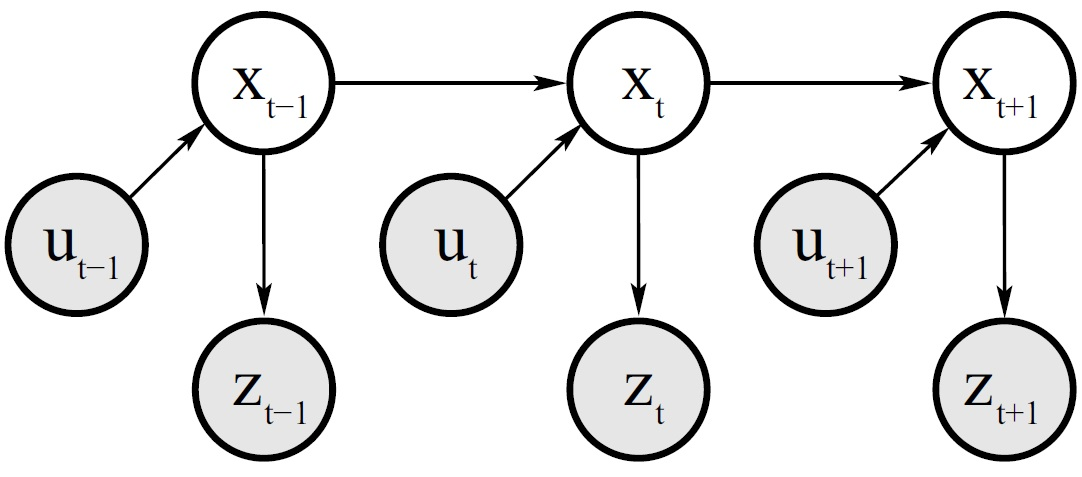
\includegraphics[width=0.8\linewidth]{22orig}}
 	\caption{ ( Рис. 2.2. Динамическая байесовская сеть, характеризующая эволюцию управления, состояний и измерений.)}
 	\label{fig:22orig}
 \end{figure}
  
 Это обсуждение раскрывает смысл двух результирующих условных вероятностей: $p(x_t | x_{t-1}, u_t)$ и $p(z_t | x_t)$. Вероятность $p(x_t | x_{t-1}, u_t)$\\
 ВЕРОЯТНОСТЬ
 ПЕРЕХОДА СОСТОЯНИЙ\\
 называется \textit{вероятностью перехода состояний}. Она определяет изменение состояния среды со временем в виде функции от управления роботом $u_t$. Окружающие среды робота имеют стохастический характер, поэтому $p(x_t | x_{t-1}, u_t)$ представляет собой вероятностное распределение, а не детерминированную функцию. В некоторых случах распределение вероятности перехода состояний не зависит от временного индекса $t$, и в этом случае можно написать $p(x' | u, x)$, где $x'$ последующее, а $x$ – предыдущее состояние.\\
 ВЕРОЯТНОСТЬ ИЗМЕРЕНИЯ 
  
 Вероятность $p(z_t | x_t)$ называется \textit{вероятностью измерения}. Она также может не зависеть от показателя времени $t$, и, в этом случае, записываться как $p(z |x)$. Вероятность измерения определяет вероятностное соотношение, согласно которому измерения $z$ генерируются из окружающей среды с состоянием $x$. Справедливо считать измерения зашумленными проекциями состояния.
  
 Динамическая стохастическая система, состоящая из робота и его окружения описываются вероятностями перехода состояний и измерений. На Рис. 2.2 показаны развитие состояний и измерений, определённых этими вероятностями. Состояние в момент времени $t$  стохастически зависимо от состояния в момент времени ${t-1}$ и управления $u_t$. Измерение $z_t$ стохастически зависит от состояния в момент времени $t$. Такая временная генеративная модель также известна как \textit{скрытая марковская модель} 
 (hidden Markov model -HMM) или \textit{динамическая байесовская сеть} (dynamic Bayes network -DBN).\\
 
\textbf{ 2.3.4 Распределения оценок}\\

 ОЦЕНКА
 
 Другой ключевой концепцией вероятностной робототехники является оценка. Оценка отражает внутреннюю осведомлённость робота о состоянии окружающей среды. Мы уже говорили, что состояние невозможно измерить напрямую.  Например, положение робота может быть обозначено как $\langle x_t = 14.12, 12.7, 45^o\rangle$ в некоторой глобальной системе координат, но своего настоящего положения он, обычно, определить неспособен, поскольку положение невозможно измерить напрямую (даже с помощью GPS!). Вместо этого, робот вынужден делать \textit{заключение} о своём положении на основании данных. Таким образом, необходимо разделять настоящее состояние и внутреннюю оценку этого состояния.\\
 ИНФОРМАЦИОННОЕ СОСТОЯНИЕ\\ 
 Синонимами оценки в литературе являются термины \textit{«знание о состоянии»} (state of knowledge) и \textit{«информационное состояние»} (information state) (не путать с информационным вектором и информационной матрицей, которые будут обсуждаться ниже).
 
 В вероятностной робототехнике оценки рассматриваются через распределения условной вероятности. Распределение оценки назначает вероятность (или значение плотности) для каждой возможной гипотезы относительно реального состояния. Распределения оценок являются апостериорными вероятностями переменных состояния, вычисленными на основании доступных данных. Условимся обозначать оценку переменной состояния $x_t$ как $bel(x_t)$, в качестве сокращения для апостериорной вероятности\\

 (2.33) $$bel(x_t) = p(x_t | z_{1:t}, u_{1:t})$$
 Апостериорная вероятность  - это вероятностное распределение по состоянию $x_t$ в момент времени $t$, вычисленная на основании всех прошлых измерений $z_{1:t}$ и всех прошлых действий управления $u_{1:t}$.
 
 Читатель может заметить, что оценка производится \textit{после} получения измерения $z_t$. Время от времени более полезным будет вычислить апостериорную вероятность сразу после выполнения управляющего действия $u_t$, но \textit{до} включения в расчёт $z_t$. 
 Такая апостериорная оценка будет иметь следующий вид:\\

 (2.34) $$\overline{bel}(x_t) = p(x_t | z_{1:t-1}, u_{1:t})$$
 
 ПРОГНОЗ\\
 Такое вероятностное распределение в контексте вероятностной фильтрации часто обозначается как \textit{«прогноз»}. Этот термин отражает факт того, что $\overline{bel}(x_t)$ «прогнозирует» состояние в момент времени $t$, основываясь на предыдущих апостериорных состояниях, но до принятия в расчёт измерения в момент времени $t$.  Вычисление $bel(x_t)$ из $\overline{bel}(x_t)$  называется коррекцией или обновлением измерения\\
 
 \textbf{2.4 Байесовские фильтры}\\
 
 \textbf{2.4.1 Алгоритм байесовского фильтра}\\

 ФИЛЬТР БАЙЕСА
 
 Самый общий алгоритм для вычисления оценок – это алгоритм \textit{байесовского фильтра}. Этот алгоритм позволяет вычислить распределение оценок $bel$ на основе данных измерения и управления. Рассмотренный в начале базовый алгоритм будет сначала проиллюстрирован на примере, а, затем мы выведем его математическим путём на основании сделанных допущений.
  
 В Таблице 2.1 в псевдо-алгоритмической форме приведён основной алгоритм байесовского фильтра. Байесовский фильтр рекурсивный, поэтому оценка $bel(x_t)$ в момент времени $t$ вычислена\\ 
 {}\\
  \begin{table}[h]
 	\begin{center}
 		\begin{tabular}{|l|}
 			\hline
 			{}\\
 			1: \hspace{3mm} Algorithm Bayes\_filter $(bel(x_{t-1}), u_t, z_t):$ \\
 			2: \hspace{6mm} \textit{for all} $x_t$ \textit{do} \\
 			3: \hspace{9mm} $\overline{bel}(x_t) =\int p(x_t | u_t, x_{t-1}) bel(x_{t-1}) dx_{t-1}$ \\
 			4: \hspace{9mm} $bel(x_t) =\eta p(z_t | x_t)\overline{bel}(x_t)$\\
 			5: \hspace{6mm} \textit{endfor}\\
 			6: \hspace{3mm} \textit{return} $bel(x_t)$\\
 			{}\\
 			\hline
 		\end{tabular}
 	\caption{(Таблица 2.1 Общий алгоритм байесовской фильтрации.)}
 	\end{center}
 \end{table}\\
 
 на основании оценки $bel(x_{t-1})$ для момента времени ${t-1}$. На вход поступает оценка $bel$ в момент времени ${t-1}$, наряду с последним значением управления $u_t$ и последним измерением  $z_t$. На выходе  вычисляется значение оценки $bel(x_t)$ в момент времени $t$. В Таблице 2.1 приведена одна итерация алгоритма байесовского фильтра: \textit{правило обновления}.\\
 ОБНОВЛЕНИЕ ДЛЯ БАЙЕСОВСКОГО ФИЛЬТРА\\
 Обновление применяется рекурсивно, для того, чтобы вычислить оценку $bel(x_t)$ из предварительно вычисленной оценки $bel(x_{t-1})$.
 
 Алгоритм байесовского фильтра последовательно проходит два важных шага. В строке 3 обрабатывается управляющее воздействие $u_t$. Это происходит через оценку состояния по $x_t$ на основе предыдущей оценки по состоянию $x_{t-1}$ и управляющему воздействию $u_t$. В частности, оценка
 $\overline{bel}(x_t)$ перехода робота в состояние $x_t$, получается интегрированием (фактически, суммированием) произведений двух распределений: априорного, полученного для $x_{t-1}$, и вероятности того, что управляющее воздействие $u_t$ вызовет переход от $x_{t-1}$ к $x_t$. Читатель может заметить схожесть такта обновления с Выражением (2.12). Как было сказано ранее, этот такт обновления называется обновлением управления или \textit{прогнозом}.\\
  
 Второй такт работы байесовского фильтра называется \textit{обновлением измерения}. В строке 4 алгоритма выполняется умножение оценки $\overline{bel}(x_t)$ на вероятность того, что будет обнаружено наблюдение $z_t$. Это действие повторяется для каждого гипотетического апостериорного состояния $x_t$. Как станет очевидным далее, при выводе основных равенств алгоритма фильтрации, результирующее произведение, вообще-то, вероятностью не является, и может не интегрироваться до 1. В силу этого, результат необходимо нормализовать с помощью нормализующего члена $\eta$. Это даёт итоговую оценку $bel(x_t)$, значение которой и возвращается в строке 6 алгоритма.
 
 Для рекурсивного вычисления апостериорной оценки, алгоритму требуется начальная оценка $bel(x_0)$ в момент времени $t = 0$ в качестве граничного условия. Если известно точное значение $x_0$, $bel(x_0)$ следует инициализировать переменную, сконцентрировав вероятность на верном значении $x_0$, и\\
 
 \begin{figure}[h]
 	\center{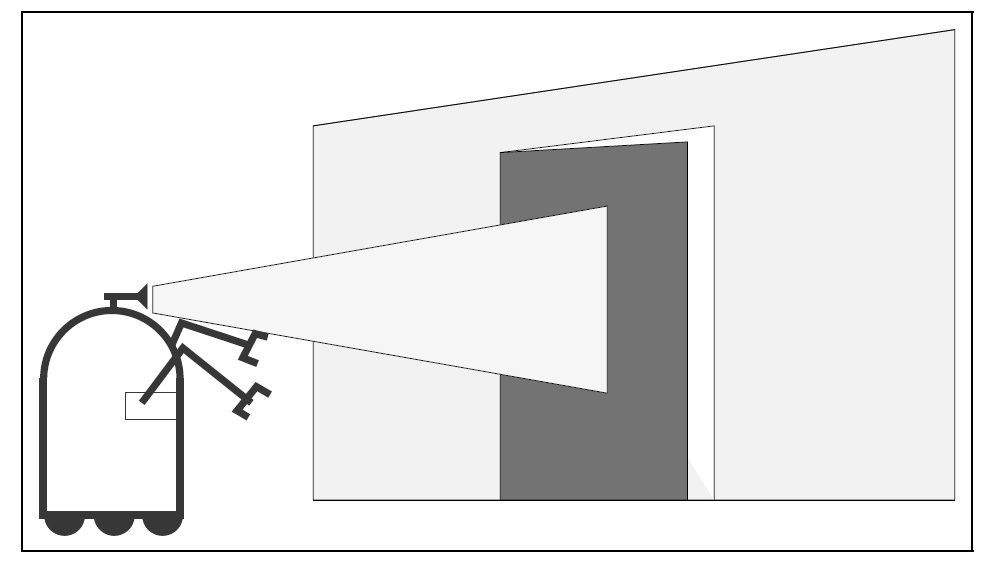
\includegraphics[width=0.8\linewidth]{23orig}}
 	\caption{ (  Рис. 2.3 Мобильный робот определяет состояние двери.)}
 	\label{fig:23orig}
 \end{figure}
 установив нуль во всех остальных точках. Если же значение $x_0$ совершенно неизвестно, оценку $bel(x_0)$ можно инициализировать равномерным распределением в окрестности $x_0$ (или применимым распределением Дирихле). Частичную информацию о значении $x_0$ возможно выразить с помощью неравномерного распределения, хотя на практике наиболее часто встречаются именно эти два случая полной осведомлённости или полного незнания.
  
 В приведённой форме алгоритм байесовского фильтра пригоден только для очень простых оценочных задач. В частности, необходимо или гарантировать закрытую форму интегрирования в строке 3 и умножения в строке 4, или ограничиться конечными пространствами состояний, чтобы интеграл в строке 3 свёлся к конечной сумме.\\ 
 
 \textbf{2.4.2 Пример}\\
 
 Наша иллюстрация алгоритма байесовской фильтрации основана на сценарии из Рис. 2.3, где показан робот, который оценивает состояние двери с помощью камеры.  Чтобы упростить задачу, давайте предположим, что дверь может быть только в одном из двух возможных состояний, открытом или закрытом, при этом только робот может изменить ее состояние. Допустим также, что, изначально, робот ничего не знает о текущем состоянии двери. Чтобы выразить это, назначим равную априорную вероятность для двух возможных состояний двери:\\ 
 $bel(X_0=\mbox{is\_open}) = 0,5$\\
 $bel(X_0=\mbox{is\_closed} = 0,5$\\
 Также допустим, что датчики робота подвержены зашумлению. Шум характеризуется следующими условными вероятностями:\\
 $p(Z_t =\mbox{sense\_open} | X_t =\mbox{is\_open}) = 0,6$\\ 
 $p(Z_t = \mbox{sense\_closed} | X_t =\mbox{is\_open}) = 0,4$\\
 и\\
 $p(Z_t =\mbox{sense\_open} | X_t =\mbox{is\_closed}) = 0,2$\\
 $p(Z_t =\mbox{sense\_closed} | X_t =\mbox{is\_closed} ) = 0,8$\\
 Очевидно, что датчики робота довольно надёжно распознают закрытую дверь, и вероятность ошибки составляет 0,2. Однако, когда дверь открыта, имеется существенная вероятность ошибочного измерения, равная 0,4 .
 
 И, наконец, давайте допустим, что робот может толкать дверь манипулятором, чтобы открыть ее. Если дверь уже была открыта, она остаётся открытой. Если же она была закрыта, после действия манипулятором робота она откроется с вероятностью 0,8:\\
 $p(X_t =\mbox{is\_open} | U_t =\mbox{push}, X_{t\_1} =\mbox{is\_open}) = 1$\\
 $p(X_t =\mbox{is\_closed}  | U_t =\mbox{push} , X_{t\_1} =\mbox{is\_open}) = 0$\\
 $p(X_t =\mbox{is\_open}  | U_t =\mbox{push} , X_{t\_1} =\mbox{is\_closed} ) = 0.8$\\
 $p(X_t =\mbox{is\_closed}  | U_t =\mbox{push} , X_{t\_1} =\mbox{is\_closed} ) = 0.2$\\
 Робот также может принять решение не использовать манипулятор, и тогда состояние окружающего мира не меняется. Этот случай описывается следующими вероятностями:\\
 $p(X_t =\mbox{is\_open}  | U_t = \mbox{do\_nothing}, X_{t\_1} = \mbox{is\_open}) = 1$\\
 $p(X_t =\mbox{is\_closed}  | U_t =\mbox{do\_nothing} , X_{t\_1} =\mbox{is\_open} ) = 0$\\
 $p(X_t =\mbox{is\_open}  | U_t =\mbox{do\_nothing} , X_{t\_1} = \mbox{is\_closed}) = 0$\\
 $p(X_t =\mbox{is\_closed}  | U_t =\mbox{do\_nothing} , X_{t\_1} =\mbox{is\_closed} ) = 1$\\
 Допустим, в момент времени $t = 1$, робот не выполняет никаких управляющих действий, но обнаруживает открытую дверь. В результате, апостериорная оценка вычисляется байесовским фильтром, используя в качестве входных значений априорную оценку $bel(X_0)$, управляющее воздействие $u1 = \mbox{do\_nothing}$, и измерение $\mbox{sense\_open}$. Поскольку пространство состояний конечно, интеграл в строке 3 сводится до конечной суммы:\\ 
 $\overline{bel}(x_1)$\\
 $= \int p(x_1 | u_1, x_0) bel(x_0) dx_0$\\
 $=\sum_{x_0} p(x_1 | u_1, x_0) bel(x_0)$\\
 $= p(x_1 | U_1 = \mbox{do\_nothing}, X_0 =\mbox{is\_open} ) bel(X_0 =\mbox{is\_open} )\\ + p(x_1 | U_1 = \mbox{do\_nothing}, X_0 =\mbox{is\_closed} ) bel(X_0=\mbox{is\_closed})$\\
 {}\\
 Теперь можно заменить два возможных значения переменной состояния $X_1$. Для гипотезы $X_1=\mbox{is\_open}$, получаем\\
 $\overline{bel}(X_1 =\mbox{is\_open})\\
 = p(X_1 =\mbox{is\_open}  | U_1 =\mbox{do\_nothing} , X_0 =\mbox{is\_open} ) bel(X_0 =\mbox{is\_open} )\\
 + p(X_1 =\mbox{is\_open}  | U_1 =\mbox{do\_nothing} , X_0 =\mbox{is\_closed} ) bel(X_0 =\mbox{is\_closed} )\\
 = 1\times0.5 + 0\times0.5 = 0.5$\\
 {}\\
 Аналогично, для $X_1 =\mbox{is\_closed}$  получается\\
 $\overline{bel}(X_1 =\mbox{is\_closed} )\\
 = p(X_1 =\mbox{is\_closed}  | U_1 =\mbox{do\_nothing} , X_0 =\mbox{is\_open} ) bel(X_0 =\mbox{is\_open} )\\
 + p(X_1 =\mbox{is\_closed}  | U_1 =\mbox{do\_nothing} , X_0 =\mbox{is\_closed} ) bel(X_0 =\mbox{is\_closed} )\\
 = 0\times0.5 + 1\times0.5 = 0.5$\\
 {}\\
 Факт равенства оценки $\overline{bel}(x_1)$ и априорной оценки $bel(x_0)$ не должен удивлять, поскольку действие $\mbox{do\_nothing}$ не влияет на состояние окружающего мира, а сам окружающий мир в нашем примере неизменен по времени.
  
 Однако, когда в расчёт принимается измерение, оценка изменяется. В строке 4 алгоритма байесовского фильтра\\
 {}\\
 $bel(x_1) =\eta p(Z_1 =\mbox{sense\_open}  | x_1) \overline{bel}(x_1)$\\
 {}\\
 Для двух возможных случаев, $X_1 =\mbox{is\_open}$ и $X_1 =\mbox{is\_closed}$, получаем\\
 $bel(X_1 =\mbox{is\_open} )\\
 =\eta p(Z_1 =\mbox{sense\_open}  | X_1 =\mbox{is\_open} ) \overline{bel}(X_1 =\mbox{is\_open} )\\
 = \eta 0.6\times0.5 =\eta 0.3$\\
 {}\\
 и, соответственно\\
 $bel(X_1 =\mbox{is\_closed} )\\
 =\eta p(Z_1 =\mbox{sense\_open}  | X_1 =\mbox{is\_closed} ) \overline{bel}(X_1 =\mbox{is\_closed} )\\
 = \eta 0.2\times0.5 = \eta 0.1$\\
 {}\\
 Теперь легко вычислить нормализующий член $\eta$:\\
 $\eta = (0.3 + 0.1)^{-1} = 2.5$\\
 {}\\ 
 Отсюда, получаем:\\
 $bel(X_1 =\mbox{is\_open} ) = 0.75$\\
 $bel(X_1 =\mbox{is\_closed}) = 0.25$\\
 {}\\
 Эти вычисления очень просто повторяются на следующем такте времени. Как читатель может убедиться, для $u_2 =\mbox{push}$  и $z_2 =\mbox{sense\_open}$, получаем\\
 {}\\
 $\overline{bel}(X_2 =\mbox{is\_open} ) = 1\times0.75 + 0.8\times0.25 = 0.95$\\
 $\overline{bel}(X_2 =\mbox{is\_closed} ) = 0\times0.75 + 0.2\times0.25 = 0.05$\\
 и\\
 $bel(X_2 =\mbox{is\_open} ) =\eta 0.6\times0.95\approx0.983$\\
 $bel(X_2 =\mbox{is\_closed} ) =\eta0.2\times0.05\approx0.017$\\
 {}\\
 К этому моменту оценка робота указывает на то, что, дверь открыта с вероятностью 0,983.
 
 На первый взгляд, эта вероятность может показаться достаточно большой, чтобы просто принять эту гипотезу в качестве состояния окружающего мира и действовать соответствующим образом. Однако, такой подход может стать неоправданно дорогим. Если ошибка перепутать закрытую дверь с открытой имеет цену (например, робот врежется в закрытую дверь), очень важно принять во внимание обе гипотезы, какой бы невероятной одна из них не была. Просто представьте, каково будет лететь на самолёте, автопилот которого способен избежать катастрофы с вероятностью 0,983!\\

 \textbf{ 2.4.3 Математический вывод для байесовского фильтра}\\
 
 Продемонстрируем правильность алгоритма байесовской фильтрации с помощью индукции. Чтобы это сделать, необходимо показать, что он верно вычисляет апостериорное распределение $p(x_t | z_{1:t}, u_{1:t})$ из соответствующего апостериорного же распределения $p(x_{t-1} | z_{1:t-1}, u_{1:t-1})$, но взятого на один такт ранее. Правильность доказывается с помощью индукции при условии верной инициализации априорной оценки $bel(x_0)$ в момент времени $t = 0$.
 
 Для вывода требуется, чтобы состояние $x_t$ было полным, как было определено в Главе 2.3.1, а управляющие воздействия – выбирались случайным образом. Первый этап нашего вывода включает применение формулы Байеса (2.16) к целевой апостериорной вероятности:\\
 
 (2.35)$$p(x_t | z_{1:t}, u_{1:t}) = \frac{p(z_t | x_t, z_{1:t-1}, u_{1:t}) p(x_t | z_{1:t-1}, u_{1:t})}{p(z_t | z_{1:t-1}, u_{1:t})}$$
 
 $$=\eta p(z_t | x_t, z_{1:t-1}, u_{1:t}) p(x_t | z_{1:t-1}, u_{1:t})$$
 Теперь используем допущение о том, что состояние полное. В Главе 2.3.1, мы определили $x_t$ как полное, если никакие переменные до $x_t$ не могут повлиять на стохастическую эволюцию будущих состояний. В частности, если мы (предположительно) знаем состояние $x_t$, и заинтересованы в предсказании измерения $z_t$, никакие измерения или управляющие действия  не предоставят дополнительной информации. Математически это можно выразить следующей условной независимостью:\\
 
 (2.36) $$p(z_t | x_t, z_{1:t-1}, u_{1:t}) = p(z_t | x_t)$$
 Это утверждение – ещё один пример условной независимости. Оно позволяет упростить (2.35) следующим образом:\\
 
 (2.37) $$p(x_t | z_{1:t}, u_{1:t}) = \eta p(z_t | x_t) p(x_t | z_{1:t-1}, u_{1:t})$$
 и получить\\
 
 (2.38) $$bel(x_t) = \eta p(z_t | x_t) \overline{bel}(x_t)$$
 Это равенство используется в строке 4 алгоритма байесовского фильтра в Таблице 2.1.\\
 Далее, расширим значение $\overline{bel}(x_t)$, используя (2.12):\\

 (2.39) $$\overline{bel}(x_t) = p(x_t | z_{1:t-1}, u_{1:t})$$
 $$= \int p(x_t | x_{t-1}, z_{1:t-1}, u_{1:t}) p(x_{t-1} | z_{1:t-1}, u_{1:t}) dx_{t-1}$$
 И снова используется допущение о том, что состояние – полное. Это предполагает, что, если мы знаем $x_{t-1}$, прошлые измерения и действия управления не дают дополнительной информации относительно состояния $x_t$. Это позволяет\\
 
 (2.40) $$p(x_t | x_{t-1}, z_{1:t-1}, u_{1:t}) = p(x_t | x_{t-1}, u_t)$$
   Переменная $u_t$ сохраняется, поскольку она не относилась к состоянию $x_{t-1}$.
 Фактически, читатель может быстро убедиться, что $p(x_t | x_{t-1}, u_t)\neq p(x_t | x_{t-1})$.
 
 Наконец, заметим, что переменную управляющего воздействия для случайно выбранных управляющих воздействий $u_t$ можно исключить из набора условных переменных в $p(x_{t-1} | z_{1:t-1}, u_{1:t})$.\\
 Это даёт рекурсивно обновляемое равенство\\
  
 (2.41) $$\overline{bel}(x_t) = \int p(x_t | x_{t-1}, u_t) p(x_{t-1} | z_{1:t-1}, u_{1:t-1}) dx_{t-1}$$
 Легко убедиться, что это же выражение используется в строке 3 алгоритма байесовской фильтрации, приведённого в Таблице 2.1.
 
 Подведём итог. Байесовский алгоритм фильтра вычисляет апостериорную вероятность по состоянию $x_t$, при условии наличия данных измерений и управления вплоть до момента времени $t$. Вывод подразумевает, что окружающий мир задан согласно марковской модели, а, значит, состояние полное.  Любая практическая реализация этого алгоритма требует трёх вероятностных распределений: первоначальной оценки $p(x_0)$, вероятности измерения $p(z_t | x_t)$, и вероятности изменения состояния $p(x_t | u_t, x_{t-1})$.
 Мы ещё не определили эти плотности для реальных робототехнических систем, но скоро это сделаем: Глава 5 полностью посвящена $p(x_t | u_t, x_{t-1})$, а Глава 6 - $p(z_t | x_t)$. Нам также понадобится выражение для оценки $bel(x_t)$, которое будет обсуждаться в Главах 3 и 4.\\
 
\textbf{ 2.4.4 Марковское свойство}\\

 МАРКОВСКОЕ СВОЙСТВО\\
 
 Настало время рассказать о \textit{марковском свойстве} или \textit{свойстве полного состояния}, поскольку оно играет фундаментальную роль в материале, представленном в книге. 
 Марковское свойство постулирует независимость прошлых и будущих данных, если известно текущее состояние $x_t$. Чтобы увидеть, насколько важно это свойство, вернёмся к нашему примеру локализации мобильного робота. Напомним, что $x_t$ – это расположение робота, а   для оценки местоположения на неизменяемой карте используются байесовские фильтры. Марковское свойство может нарушаться в результате воздействия на датчик следующих факторов:\\
 
 • часть динамики окружающей среды не была смоделирована и не включена в $x_t$ (например, движущиеся люди и эффекты их действия на измерения датчиков в нашем примере локализации),\\
 
 • неточности вероятностных моделей $p(z_t | x_t)$ и $p(x_t | u_t, x_{t-1})$ (например, ошибки в карты для определения местоположения робота)\\
 
 • ошибки аппроксимации при использовании приблизительных представлений функций оценки (например, сетки или гауссовы функции, которые будут обсуждаться ниже), а также\\
 
 • программные переменные в управляющем программном обеспечении робота, которые влияют на несколько управляющих действий (например, переменная «расположение цели» обычно влияет на всю последовательность управляющих команд).\\
 
 В принципе, многие из этих переменных могут быть включены в представления состояния. Однако, представления неполного состояния часто предпочтительны более полным из-за уменьшения вычислительной сложности алгоритма байесовского фильтра. На практике байесовские фильтры показывают удивительную устойчивость к такого рода нарушениям. 
 При определении состояния $x_t$ рекомендуется уделить этому вопросу особое внимание, поскольку не включённые в модель переменные могут вызывать непредсказуемые, почти случайные эффекты.\\ 
 
 \textbf{2.5 Представление и вычисление}\\
 
 В вероятностной робототехнике байесовские фильтры применяются несколькими разными способами. Как мы увидим в двух следующих главах, существует достаточно много разнообразных методов и алгоритмов на основе байесовского фильтра. Каждый из этих методов основан на различных допущениях относительно вероятностей измерений и перехода состояний, а также первоначальной оценки. Используя эти допущения, порождаются разнообразные типы апостериорных распределений для алгоритмов, отличающихся вычислительными характеристиками.  В общем и целом, точные методы вычислений оценок существуют только для очень узких задач и, почти всегда, оценки предстоит аппроксимировать. Способ этой аппроксимации оказывает определяющее воздействие на сложность алгоритма. Нахождение подходящего способа аппроксимации представляет собой весьма сложную проблему, в которой нет единого универсального решения для всех задач робототехники.
 
 При выборе аппроксимации приходится находить баланс между несколькими показателями:\\
 
 1. \textbf{Вычислительная эффективность.} Некоторые способы аппроксимации, такие как линейные гауссовские методы, которые будут обсуждаться ниже, дают возможность вычисления оценки за время, кратное размерности пространства состояний. Другие алгоритмы могут потребовать времени, экспоненциально зависящего от размерности. Настраиваемые методы многочастичной фильтрации имеют переменную характеристику затрат времени, позволяя жертвовать точностью ради вычислительной эффективности.\\
  
 2. \textbf{Точность аппроксимации.} Некоторые виды приближения могут аппроксимировать широкий набор распределений с большей точностью. Например, линейное гауссовское приближение ограничено одномодальными распределениями, а частотные представления способны аппроксимировать мультимодальные распределения, хотя и с потерей точностью. Многочастичные представления дают возможность аппроксимации в широком диапазоне распределений, но количество частиц, необходимых для получения требуемой точности, может быть весьма большим.\\
 
 3. \textbf{Простота использования.} Трудность применения вероятностных алгоритмов на практике зависит от целого ряда факторов, таких, как форма записи вероятности измерения $p(z_t | x_t)$ и вероятности перехода состояния $p(x_t |u_t, x_{t-1})$. Многочастичные представления для сложных нелинейных систем часто имеют удивительно простые  реализации, что является одной из причин их сегодняшней популярности.\\ 

 В следующих двух главах будут представлены конкретные алгоритмы реализации, которые довольно сильно различаются по описанным выше критериям.\\
 
\textbf{ 2.6 Выводы}\\

 В этом разделе была представлена общая идея использования в робототехнике байесовских фильтров для оценки состояния окружающей среды и робота.\\
  
 • Взаимодействие робота с окружающей средой смоделировано в виде связанной динамической системы, в которой робот управляет окружающей средой путём выбора управляющих действий и воспринимает ее характеристики с помощью датчиков.\\
 
 • В вероятностной робототехнике динамика робота и окружающей среды описывается в виде двух вероятностных закономерностей: распределения перехода между состояниями и распределение измерения. Распределение перехода между состояниями показывает зависимость изменения  состояния в результате управляющих действий со временем. Распределение измерений показывает, каким образом измерения зависят от состояния. Оба правила имеют вероятностную природу и позволяют принимать в расчёт изначальную неопределённость в оценке состояния и восприятия.\\
 
 • \textit{Оценка} робота – это апостериорное распределение по состоянию в окружающей среде (включая состояние робота) на основании всех прошлых измерений и управляющих действий. 
 \textit{Байесовский фильтр} представляет собой основной алгоритм для вычисления оценки в робототехнике. Он имеет рекурсивную природу: оценка в момент времени $t$ вычисляется на основе оценок в предыдущий момент времени ${t-1}$.\\
  
 • Байесовский фильтр основан на \textit{марковском свойстве}, согласно которому текущее состояние является полным описанием всех прошлых. Это допущение предполагает, что оценка достаточно полно отображает все произошедшее с роботом. В робототехнике марковское свойство обычно является лишь приближением и есть определённые условия, при которых оно нарушается.\\
 
 • Поскольку байесовский фильтр не является практическим алгоритмом и, в таком виде, не может быть реализован на компьютере, вероятностные алгоритмы используют управляемые приближения. Эти приближения могут быть оценены по различным критериям, например, точности, эффективности и простоте реализации.\\
 В следующих двух главах мы обсудим два популярных семейства рекурсивных методов оценки состояния на основе байесовского фильтра.\\
 
 \textbf{2.7 Библиографические сведения}\\
 
 Базовый материал по статистике из этой главы освещается в большинстве учебников начального уровня по статистике и теории вероятности. Некоторые ранние классические тексты ДеГрута ( DeGroot, 1975), Сабраманиана (Subrahmaniam, 1979) и Торпа (Thorp, 1966) позволяют очень быстро овладеть основными понятиями. Подробности можно найти в работах Феллера, Каселла и Бергера, Таннера (Feller 1968; Casella и Berger 1990; Tanner 1996), а также Девро и Дуда (Devroye et al. 1996; Duda et al. 2000). Общепринятая в робототехнике парадигма взаимодействия робота с окружающей средой обсуждается с точки зрения категорий искусственного интеллекта Расселом и Норвигом (Russell and Norvig, 2002).\\

 \textbf{2.8 Упражнения}\\
 
 1. Робот использует датчик, определяющий расстояния в диапазоне 0-3 м. Для простоты, допустим, что реальные значения расстояния равномерно распределены в этом интервале. К сожалению, датчик может быть неисправен. При неисправности датчика постоянно выдаются значения менее 1 м, вне зависимости от реального расстояния до объекта в конусе измерения робота. Известно, что априорная вероятность неисправности датчика $p = 0,01$. \\
 Допустим, робот запрашивает датчик $N$ раз, и каждое полученное значение измерения составляет менее 1м. Какова апостериорная вероятность неисправности датчика для $N = 1, 2, . . . , 10$? Сформулируйте соответствующую вероятностную модель.\\
 2. Допустим, мы проживаем в месте, где погода в течение дня может быть только солнечной, облачной или дождливой. Функция изменения погоды представляет собой цепь Маркова со следующей таблицей переходов:\\
 \begin{table}[h]
 	\begin{center}
 		\begin{tabular}{|r|c|}
 			\hline
 			{} & Завтра будет. . . \\
 			{} & солнечно \hfill облачно \hfill дождливо \\
 			\hline
 			солнечно & 0.8\hspace{10mm} 0.2\hspace{10mm} 0 \\
 			сегодня. . .\hfill облачно &    0.4\hspace{10mm} 0.4\hspace{10mm} 0.2\\
 			дождливо & 0.2\hspace{10mm} 0.6\hspace{10mm} 0.2 \\
 			\hline
 		\end{tabular}
 	\end{center}
 \end{table}\\
{}\\

 (а) Допустим, День 1 - солнечный. Какова вероятность появления следующей последовательности дней: День 2 = \textit{облачный}, День 3 = \textit{облачный}, День 4 = \textit{дождливый}?
 
 (б) Написать программу-симулятор, которая случайным образом генерирует последовательности «погоды» из функции перехода состояний.
 
 (в) Использовать симулятор для определения стационарного распределения данной марковской цепи. Стационарное распределение измеряет вероятность того, что случайно взятый день окажется солнечным, облачным или дождливым.
 
 (г) Возможно ли определить закрытую форму решения для вычисления стационарного распределения на основании матрицы перехода состояний, приведённой выше?
  
 (д) Какова энтропия стационарного распределения?
  
 (е) Используя формулу Байеса, вычислить таблицу вероятности для вчерашней погоды по известной погоде на сегодня. (Разрешено представлять вероятности в числовом виде, а также использовать результаты предыдущих вопросов этого упражнения.)
 
 (ж) Допустим, к  модели добавили времена года. Имеющаяся функция перехода состояний выше применима только для Лета, а для Зимы, Весны и Осени используются другие функции. Нарушит ли это марковское свойство этого процесса? Объяснить ответ.\\
  
 3. Допустим, узнать погоду явным образом невозможно, и мы вынуждены полагаться на датчик. 
 Проблема состоит в том, что показания датчика зашумлены и определяются следующей моделью измерений:\\
 \begin{table}[h]
 	\begin{center}
 		\begin{tabular}{|r|c|}
 			\hline
 			{} & Показания датчика. . . \\
 			{} & солнечно \hfill облачно \hfill дождливо \\
 			\hline
 			солнечно & 0.6\hspace{10mm} 0.4\hspace{10mm} 0 \\
 			текущая погода. . .\hfill облачно &    0.3\hspace{10mm} 0.7\hspace{10mm} 0\\
 			дождливо & \hspace{1mm} 0\hspace{12mm} 0\hspace{11mm} 1 \\
 			\hline
 		\end{tabular}
 	\end{center}
 \end{table}\\
 
 (а) Допустим, День 1 солнечный (это известно точно), а в последующие четыре дня датчик показал \textit{облачно, облачно, дождливо, солнечно}. Какова вероятность, что День 5 действительно солнечный, как показывает датчик?
 
 (б) Допустим, День 1 солнечный. В течение дней 2-4 датчик показывает \textit{солнечно, солнечно, дождливо}. Для каждого из дней со второго по четвёртый, какая погода будет наиболее вероятна? Ответить на вопрос двумя способами: основываясь только на данных, доступных на нужный день, и используя перспективу, когда данные будущих дней также доступны.
  
 (в) В той же самой ситуации (День 1 солнечный, измерения для Дней 2, 3, и 4 \textit{солнечный, солнечный, дождливый}). Какая последовательность погоды для дней со второго по четвёртый наиболее вероятна? Какова вероятность для наиболее вероятной последовательности?\\
  
 4. В этом упражнении применим теорему Байеса к гауссовским распределениям. Допустим, имеется мобильный робот, который находится на длинной прямой дороге и $x$ обозначает его положение. Будем считать, что, по первоначальной оценке, робот находится на отметке $x_{init}=1000$  м, но известно, что оценка неточная. Основываясь на этой неопределённости, смоделируем первоначальную оценку для гауссовского распределения со среднеквадратичным отклонением $\sigma_{init}^2= 900 m^2$.
 
 Чтобы уточнить местоположение, запросим данные с GPS приёмника. Показания GPS $z_{GPS}= 1100$ м. Известно, что GPS приёмник имеет среднеквадратичную ошибку $\sigma_{init}^2 = 100 m^2$.\\
 
 (а)  Найдите функции плотности вероятности для априорной вероятности $p(x)$ и измерений $p(z | x)$.
  
 (б) Используя теорему Байеса, определить апостериорную вероятность $p(x | z)$. Можно ли доказать, что функция гауссова?
 
 (в) Насколько правдоподобно было априорное измерение $x_{GPS}$= 1100 м и какова вероятность ошибки GPS приёмника?\\
 Подсказка: Это упражнение на использование квадратичных выражений.\\

 5. Вывести Уравнения (2.18) и (2.19) из (2.17) и законов теории вероятности, описанных в тексте.\\

 6. Доказать Уравнение (2.25). Какие выводы можно сделать из этого выражения?\\
  
\end{document}